\documentclass{beamer}

\usepackage{graphicx,color,transparent,amsmath,url}

\useoutertheme{infolines}
\usetheme{default}
\setbeamertemplate{navigation symbols}{}

\title[Odometry and Path Following]{%
  \normalsize
  Halmstad University course DT8007\\
  Design of Embedded Intelligent Systems\\[2\baselineskip]
  \Large
  \textbf{Odometry and Path Following}\\
  for Differential-Drive Robots}
\author{Roland Philippsen}
\institute{Halmstad University}

\begin{document}

\begin{frame}[plain]
  \titlepage
  \vfill
  \begin{minipage}{\columnwidth}
    \centering
    \begin{minipage}{0.15\columnwidth}
      
\includegraphics[width=\columnwidth]{by-sa.pdf}
    \end{minipage}
    \hspace{1mm}
    \begin{minipage}{0.7\columnwidth}
      \tiny
      Except where otherwise noted,
      this work is licensed under a Creative Commons Attribution-ShareAlike 3.0 Unported License.
      \url{http://creativecommons.org/licenses/by-sa/3.0/}
    \end{minipage}
  \end{minipage}
\end{frame}



\part{Differential Drive Kinematics}

\begin{frame}
  \partpage
  \tableofcontents
\end{frame}


\section{Wheel Control}
\begin{frame}{Wheel Control}
  
  \begin{minipage}{0.3\columnwidth}
    \textbf{CPU}\\
    $\downarrow$ motor command $u$\\
    \textbf{board}\\
    $\downarrow$ motor tension [V]\\
    \textbf{motor}\\
    $\downarrow$ $\dot\beta$ [rad/s]\\
    \textbf{gear} $N_\text{w}:N_\text{m}$\\
    $\downarrow$ $\dot\beta N_\text{m} = \pm \dot\alpha N_\text{w}$\\
    \textbf{wheel} radius $R$ [m]\\
    $\downarrow v = R \dot\alpha$\\
    \textbf{velocity} [m/s]
  \end{minipage}
  \hfill
  \begin{minipage}{0.65\columnwidth}    
    \def\svgwidth{\columnwidth}
    \input{wheel-control.pdf_tex}
  \end{minipage}
  
  \vfill
  
  \begin{itemize}
  \item
    left and right wheels: subscripts l and r
  \item
    motor command (1 byte on the Pie robots) $u_\text{l,r} \leftrightarrow \dot\alpha_\text{l,r}$
  \item
    encoder counter (4 bytes on Pie) $e_\text{l,r} \leftrightarrow \alpha_\text{l,r} = \int \dot\alpha_\text{l,r} dt \approx \sum\Delta\alpha_\text{l,r}$
  \end{itemize}
  
\end{frame}


\section{Velocity and Acceleration Limits}
\begin{frame}{Velocity and Acceleration Limits}
    
  \begin{minipage}{0.55\columnwidth}
    Example: trapezoidal velocity
    \begin{align*}
      \Delta p_\text{min}
      &=
      \frac{1}{2} v \cdot t_\text{min} = \frac{v^2}{2 \cdot a_\text{max}}
      \\
      \Delta p
      &=
      p_\text{goal} - p
    \end{align*}
    
  \end{minipage}
  \hfill
  \begin{minipage}{0.4\columnwidth}
    \def\svgwidth{\columnwidth}
    \input{trapezoidal-velocity.pdf_tex}
  \end{minipage}
  
  \vfill
  
  Simplified solution sketch for $v \geq 0$ and discretized time
  \[
  v_\text{des}
  =
  \begin{cases}
    \max (v_\text{max}, v + a_\text{max} \cdot \Delta t)
    & \text{if}\; \Delta p_\text{min} < \Delta p
    \\
    v - a_\text{max} \cdot \Delta t
    & \text{otherwise}
  \end{cases}
  \]
  
  \begin{itemize}
  \item
    for negative $v$ you need to flip some signs etc
  \item
    discretized $\Delta t$ leads to problems
  \end{itemize}
  
\end{frame}


\begin{frame}{Velocity and Acceleration Limits}
  
  \textbf{Practical aspects} $\rightarrow$ discretization, lookahead, ``dead band'' \ldots

  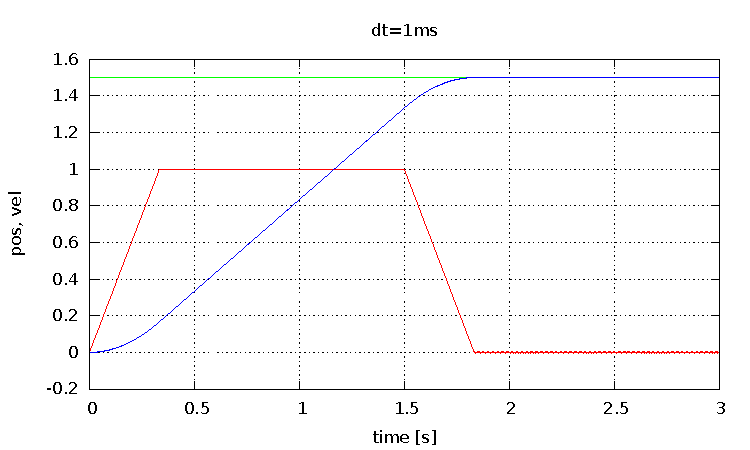
\includegraphics[width=0.5\textwidth]{p0.pdf}%
  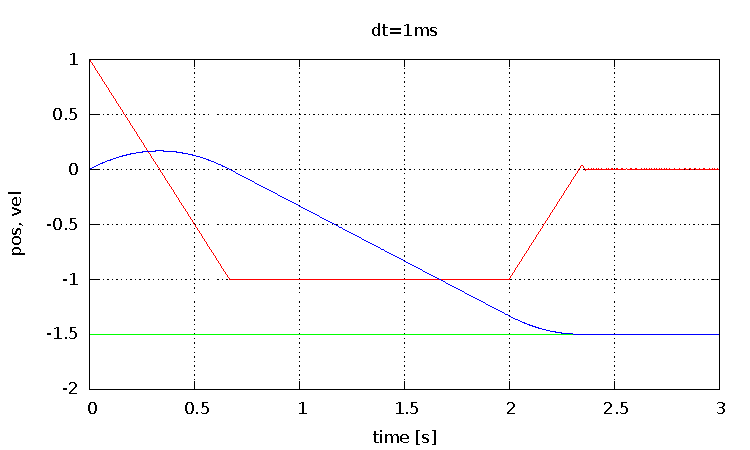
\includegraphics[width=0.5\textwidth]{p2.pdf}\\
  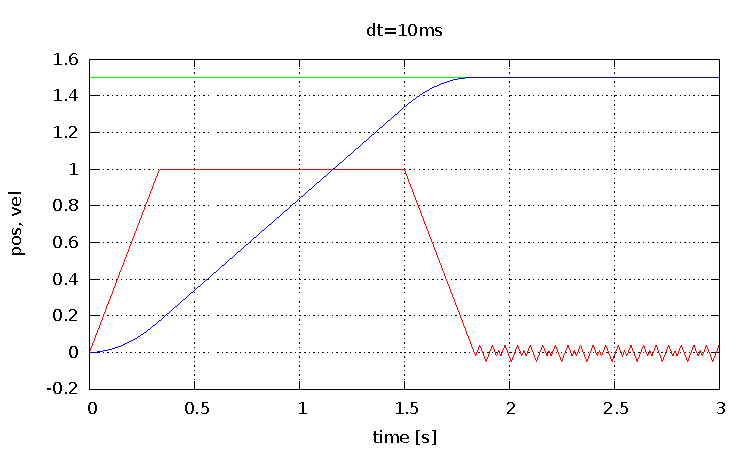
\includegraphics[width=0.5\textwidth]{p1.pdf}%
  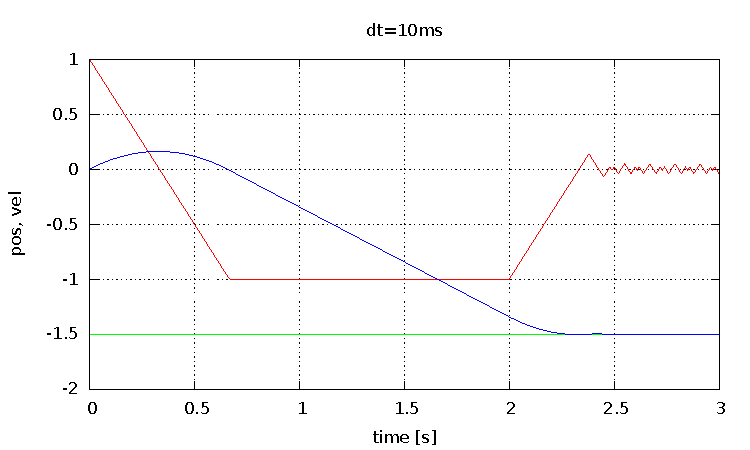
\includegraphics[width=0.5\textwidth]{p3.pdf}
  
\end{frame}


\section{Kinematics and Odometry}
\begin{frame}{Kinematics and Odometry}
  
  \begin{minipage}{0.5\columnwidth}
    In \textbf{local} frame:
    \vspace{-0.5\baselineskip}
    \begin{align*}
      \Delta\theta
      &=
      \omega \Delta t
      \\
      \Delta x
      &=
      \begin{cases}
        \text{arc} \rightarrow
        &
        S \sin \Delta \theta
        \\
        \text{else}
        &
        L \cos (\Delta \theta / 2)
      \end{cases}
      \\
      \Delta y
      &=
      \begin{cases}
        \text{arc} \rightarrow
        &
        S (1 - \cos \Delta \theta)
        \\
        \text{else}
        &
        L \sin (\Delta \theta / 2)
      \end{cases}
      \\
      \text{where}
      \\
      v_\text{l,r}
      &=
      \dot\alpha_\text{l,r} \cdot R_\text{l,r}
      \\
      v
      &=
      (v_\text{l} + v_\text{r}) / 2
      \\
      \omega
      &=
      (v_\text{r} - v_\text{l}) / B
      \\
      L
      &=
      v \Delta t
      \\
      S
      &=
      v / \omega
    \end{align*}
    
  \end{minipage}%
  \begin{minipage}{0.3\columnwidth}
    
    \def\svgwidth{1.4\columnwidth}
    \input{kinematics.pdf_tex}

    \vspace{0.5\baselineskip}
    \vspace{-0.5\baselineskip}
    \begin{align*}
      x^+
      &=
      x^- + \Delta x \cos \theta - \Delta y \sin \theta
      \\
      y^+
      &=
      y^- + \Delta y \cos \theta + \Delta x \sin \theta
      \\
      \theta^+
      &=
      \theta^- + \Delta \theta
    \end{align*}
    
  \end{minipage}
  
\end{frame}


\section{Rotate-Translate-Rotate Control}
\begin{frame}{Rotate-Translate-Rotate Control (RTR)}
    
  \centering
  \def\svgwidth{\columnwidth}
  \input{rtr.pdf_tex}
  
\end{frame}


\section{Odometry Calibration}
\begin{frame}{Odometry Calibration}
  
  Measuring the hardware parameters that influence the pose estimate.
  
  \vspace{2mm}
  
  \centering
  \fbox{\parbox{0.8\columnwidth}{
  \begin{align*}
    \Delta \theta
    &=
    \frac{\Delta p_\text{r} - \Delta p_\text{l}}{B}
    &
    \Delta p_\text{l,r}
    &=
    R_\text{l,r} \Delta \alpha_\text{l,r}
    \\
    L
    &=
    \frac{\Delta p_\text{l} + \Delta p_\text{r}}{2}
    &
    \alpha_\text{l,r}
    &=
    \frac{2 \pi N_\text{m}}{N_\text{w} N_\text{e}} e_\text{l,r}
    %
    % b * Nm = a * Nw --> a = b * Nm / Nw
    % e = b * Ne      --> b = e / Ne
    %                 --> a = e * Nm / Nw / Ne
    %
  \end{align*}}}
  
  \vspace{2mm}
  
  \begin{minipage}[t]{0.45\columnwidth}
    \textbf{1.\ determine $\bar{R} = (R_\text{l}+R_\text{r})/2$}
    \begin{align*}
      L
      &=
      \Delta\bar{p} = \bar{R} \Delta\bar{\alpha}
      \\
      &=
      (2 \pi N_\text{w} \bar{R} \Delta{\bar{e}}) / (N_\text{e} N_\text{m})
      \\
      \bar{R}
      &=
      \frac{N_\text{e} N_\text{m} L}{2\pi N_\text{w} \Delta\bar{e}}
    \end{align*}
    unknown $N$? $\rightarrow$ use $L = R^\ast\Delta{\bar{e}}$
  \end{minipage}
  \hfill
  \begin{minipage}[t]{0.45\columnwidth}
    \textbf{2.\ determine $B$}
    \begin{align*}
      B
      &=
      (\Delta p_\text{r} - \Delta p_\text{l}) / \Delta\theta
      \\
      &=
      \bar{R}(\Delta\alpha_\text{r} - \Delta\alpha_\text{l}) / \Delta\theta
      \\
      &=
      \frac{2\pi\bar{R}N_\text{w}}{N_\text{e}N_\text{m} \Delta\theta} (\Delta e_\text{r} - \Delta e_\text{l})
    \end{align*}
    try $\Delta\theta = 2k\pi$ with $k\in\mathbb{N}$
  \end{minipage}
    
\end{frame}



\begin{frame}{Take Home Message}

  Underlying control capabilities
  \begin{itemize}
  \item
    wheel speed $\dot\alpha\leftrightarrow$ motor command $u$
  \item
    acceleration \& speed limts $\leftrightarrow$ trapezoidal velocity
  \item
    RTR $v_\text{l}=\pm v_\text{r}$ good for odometry calibration
  \end{itemize}
  
  \vfill
  
  Dealing with differential-drive kinematics
  \begin{itemize}
  \item
    $\{\dot\alpha_\text{l},\dot\alpha_\text{r}\} \leftrightarrow \{v,\omega\}$ with parameters $\{R_\text{l}, R_\text{r}, B\}$
  \item
    odometry: $\{\Delta e_\text{l}, \Delta e_\text{r}\} \rightarrow \{v,\omega\} \rightarrow \{\Delta x, \Delta y, \Delta \theta\}$
  \end{itemize}
  
\end{frame}


\part{Control and Path Following}

\begin{frame}
  \partpage
  \tableofcontents
\end{frame}



\section{Odometry Calibration Revisited}
\begin{frame}{Odometry Calibration Revisited}
  
  \begin{itemize}
  \item
    inherent limitations: encoder resolution, gear backlash
  \item
    geometric simplifications, i.e. $R_\text{l} \ne R_\text{r}$
    
    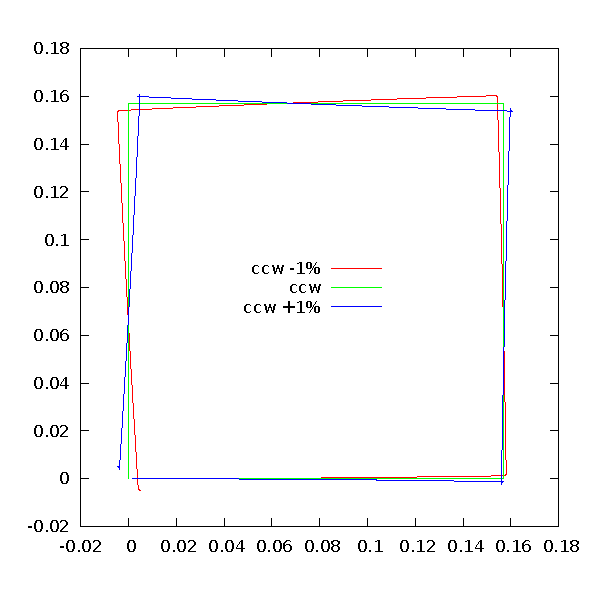
\includegraphics[width=0.4\columnwidth]{odom-ccw.pdf}%
    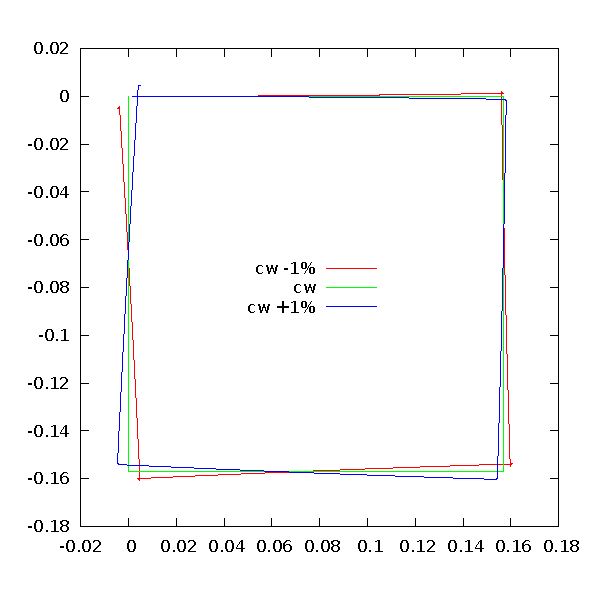
\includegraphics[width=0.4\columnwidth]{odom-cw.pdf}
    
    \url{http://www-personal.umich.edu/~johannb/umbmark.htm}
  \end{itemize}
  
\end{frame}  


\section{Pose Feedback Control}
\begin{frame}{Pose Feedback Control}
  
  \begin{minipage}{0.45\columnwidth}
    \def\svgwidth{\columnwidth}
    \input{ptctrl.pdf_tex}
  \end{minipage}
  \begin{minipage}{0.5\columnwidth}
    polar error:
    \vspace{-\baselineskip}
    \begin{align*}
      \Delta x
      &=
      x_\text{goal} - x
      \\
      \Delta y
      &=
      y_\text{goal} - y
      \\
      \epsilon
      &=
      \text{atan2}(\Delta y, \Delta x)
      \\
      \rho
      &=
      \sqrt{\Delta x^2 + \Delta y^2}
      \\
      \gamma
      &=
      \epsilon - \theta
      \\
      \delta
      &=
      \theta_\text{goal} - \gamma - \theta
      \\
      \text{with}
      &\quad
      \gamma, \delta \in (-\pi, \pi)
    \end{align*}
  \end{minipage}
  
  \vfill
  \begin{itemize}
  \item
    desired speed:
    $v = k_\rho \rho,\quad \omega = k_\gamma \gamma + k_\delta \delta$\\
    \emph{but beware of velocity limits!}
  \item
    stability:
    $k_\rho > 0,\quad k_\delta < 0,\quad k_\gamma + \frac{5}{3}k_\delta - \frac{2}{\pi}k_\rho > 0$
  \end{itemize}
  
  \hfill\tiny\emph{[Siegwart and Nourbakhsh. Introduction to Autonomous Mobile Robots. MIT Press, ISBN 0-262-19502-X.]}
\end{frame}


\section{Path Following}
\begin{frame}{Path Following}
  
  % XXXX to do: add a sketch
  
  Basic idea:
  \begin{itemize}
  \item
    $p_\text{goal}$ moves along path from $p_\text{start}$ to $p_\text{end}$
  \item
    feedback controller to the moving $p_\text{goal}$
  \end{itemize}
  
  \vfill
  
  Formulation:
  \begin{itemize}
  \item
    create a parameterized curve
    $
    q(\lambda) = \begin{bmatrix} x(\lambda) \\ y(\lambda) \end{bmatrix}
    $
  \item
    use its derivative to find $\theta(\lambda)$ and the stepsize $\Delta\lambda$
  \end{itemize}
  
\end{frame}

\begin{frame}{Spline Paths}
  
  Uniform Cubic B-Spline with 3 segments
  
  \vfill
  
  \begin{minipage}{0.4\columnwidth}
    
    \[
    q(\lambda) = \begin{cases}
      q_0(\lambda)   & \text{for} \lambda\in[0,1] \\
      q_1(\lambda-1) & \text{for} \lambda\in[1,2] \\
      q_2(\lambda-2) & \text{for} \lambda\in[2,3]
    \end{cases}
    \]
    
    Requires 6 control points $Q_i$
    \begin{itemize}
    \item
      the start pose determines $Q_0, Q_1, Q_2$
    \item
      the end pose determines $Q_3, Q_4, Q_5$
    \end{itemize}
    
  \end{minipage}
  \hfill
  \begin{minipage}{0.53\columnwidth}
    \centering
    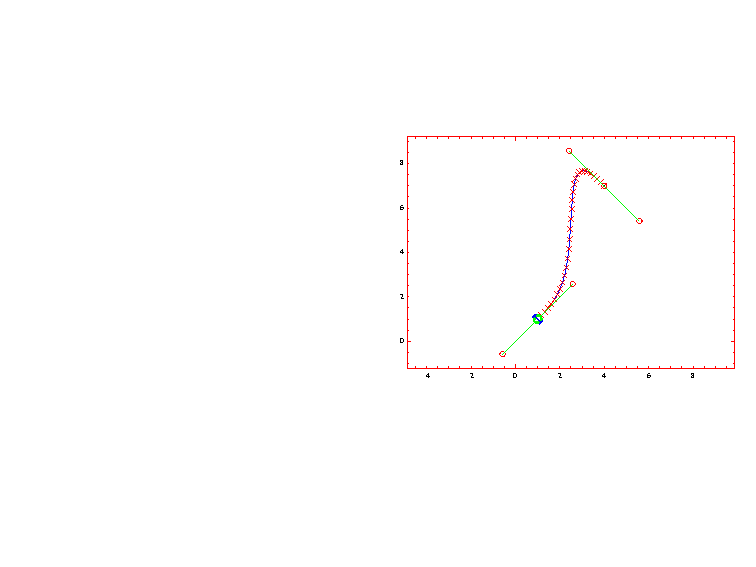
\includegraphics[width=\columnwidth]{spline-ulf-2.pdf}
  \end{minipage}
  
\end{frame}

\begin{frame}{Uniform Cubic B-Spline}
  
  Each segment is defined as follows:
  
  \begin{align*}
    q_i(\tau) &= \sum_{k=0}^{3} b_{k}(\tau) Q_{i+k}
    &
    \text{where}
    \begin{cases}
      b_0  &= (-\tau^3 + 3\tau^2 - 3\tau + 1) / 6 \\
      b_1  &= (3\tau^3 - 6\tau^2 + 4) / 6 \\
      b_2  &= (-3\tau^3 + 3\tau^2 + 3\tau + 1) / 6 \\
      b_3  &= \tau^3 / 6 \\
      \tau &\in [0,1]
    \end{cases}
  \end{align*}
  
  \begin{minipage}{0.25\columnwidth}
    \centering
    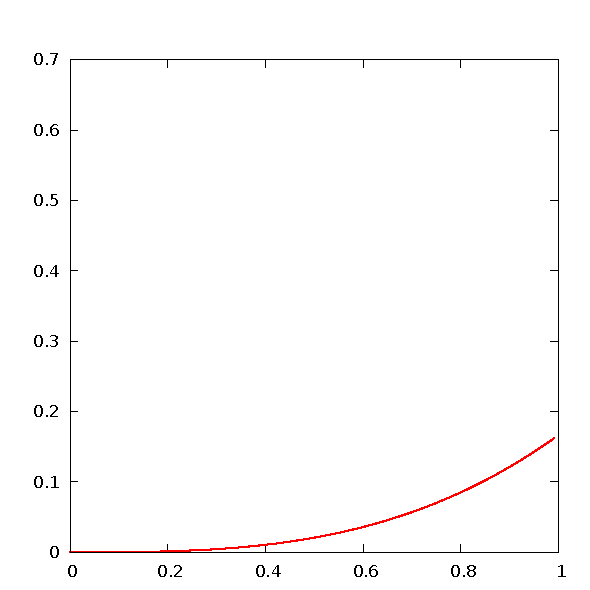
\includegraphics[width=\columnwidth]{b3.pdf}\\
    $b_3$
  \end{minipage}%
  \begin{minipage}{0.25\columnwidth}
    \centering
    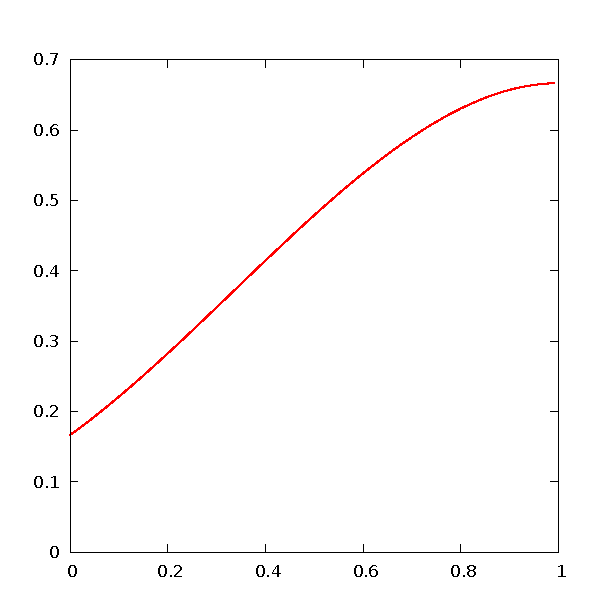
\includegraphics[width=\columnwidth]{b2.pdf}\\
    $b_2$
  \end{minipage}%
  \begin{minipage}{0.25\columnwidth}
    \centering
    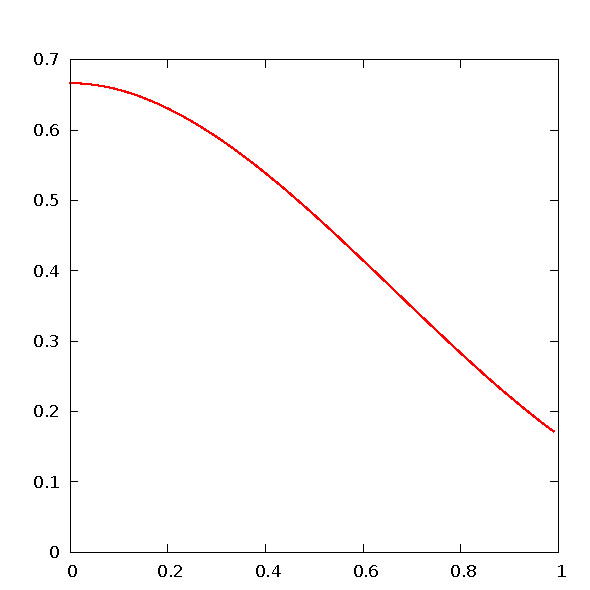
\includegraphics[width=\columnwidth]{b1.pdf}\\
    $b_1$
  \end{minipage}%
  \begin{minipage}{0.25\columnwidth}
    \centering
    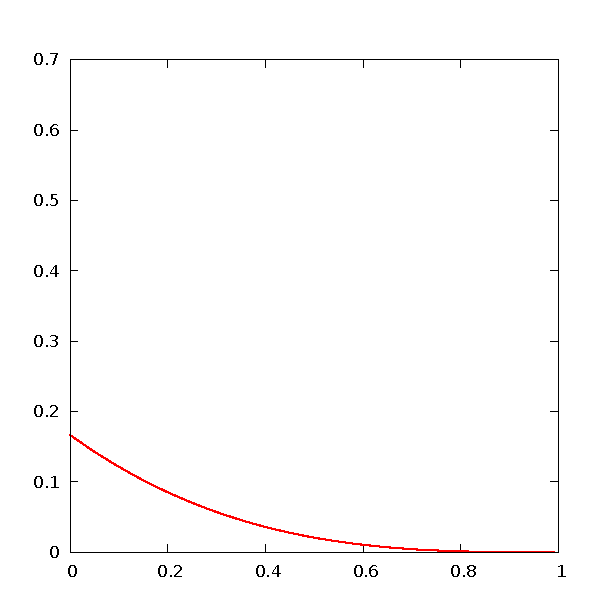
\includegraphics[width=\columnwidth]{b0.pdf}\\
    $b_0$
  \end{minipage}
  
\end{frame}



\section{Integration with Localization}
\begin{frame}{Integration with Localization}
  
  Pure odometry will not get you exactly where you want to be.
  \begin{itemize}
  \item
    uncertain pose, errors accumulate
  \item
    imperfect actuation
  \end{itemize}
  
  \vfill
  
  Use global pose information, i.e.\ overhead camera.
  \begin{itemize}
  \item
    regularly update the odometry estimate $\Rightarrow$ \textbf{sensor fusion}
  \end{itemize}

  \vfill
  
  Some of the things that make this interesting:
  \begin{itemize}
  \item
    sensor resolution and accuracy
  \item
    delays, possibly unknown and time-varying
  \item
    noise and outliers, possibly location-dependent
  \end{itemize}
  
\end{frame}


\section{Take Home Message}

\begin{frame}{Take Home Message}
  
  \begin{itemize}
  \item
    pose control: $\{\rho, \gamma, \delta\} \rightarrow \{v,\omega\}$ good for short distances
  \item
    path following via feedback control to a ``carrot'' (goal pose)
  \item
    polynomial splines can serve as paths (if done right)
    \begin{itemize}
    \item
      choosing control points
    \item
      computing tangents
    \item
      properly incrementing $\lambda$
    \end{itemize}
  \item
    the need for sensor fusion
  \end{itemize}
  
\end{frame}


\end{document}

